\chapter{Cosmology Summary}
%\chapter{Cosmology Recap}
% nel discutere le likelihood in particolare che si hanno in questi contesti è bene evidenziare le proprietà rilevanti ai fini di cosmolime - più in generale ad es. la stabilità/regolarità delle stesse che ne permette l'emulazione in primo luogo (su questo puoi trarre spunto dall'introduzione di cosmopower sicuramente)

% Similmente: dire qui che siccome i dati sono simulati sono potenzialmente infiniti? (e senza rumore, più o meno)

% citare modern cosmology et similia?

%\section{LSS}

%\section{CMB}
% \cite{likelihood_cmb} \cite{modern_cosmology}

% power spectra ubiquitous topic in cosmology, on one hand they allow for (near) lossless compression of experimental data, on the other they have a rich structure with strong dependence con cosmological parameters, hence it provides a perfect middle ground between theory and experiment that successfully allows for inference of cosmological parameters
% (quanto sopra basato da una frase del dodelson, credo)

% giocarsela sulle informazioni contenute là dentro, insomma. Inoltre quanto detto sopra sui power spectra è generale, ci concentriamo su una semplificazione del modello del cmb per dare un'idea. Lo scopo di questa sezione è apprezzare meglio perché i PS servano per fare inferenza di un certo tipo/livello e perché sia utile avere un modo per saltare i calcoli "banali" (e sicuramente pallosi)
% con questo intendo dire che di solito il grosso delle sfide sta nella parte sperimentale (sia farei satelliti che comprimere l'informazione in opportuni estimators del PS/approssimazioni della likelihood eccetera); calcolare gli spettri teorici è relativamente straightforward ma pesante, quindi rappresenta un peso morto del cavolo che vorremmo toglierci di dosso con gli emulatori del caso

% forse è meglio chiedere come procedere qui. In effetti potrebbe bastare qualcosa sulle luminosity distances e le supernove, e in effetti probabilmente era quello che intendeva il prof Raveri. Tuttavia direi che quel poco che serve è quello che è contenuto nel notebook, ed è talmente poco che potrebbe essere fornito in itinere in quel capitolo stesso...
% è anche vero che il prof Liguori ha menzionato i C_l nella chiamata, quindi sembra pertinente parlarne.

% spiegare il legame fra likelihood e power spectra è utile per capire come mai un approccio indiretto sia non solo possible ma anche sensato. Emulatori tipo cosmopower si usano per sostituire (parti del)le likelihood, ma non calcolano direttamente le likelihood... allora perché si possono usare? Per il legame di equivalenza che c'è fra likelihood e power spectra. Questo è un buon motivo per giustificare l'esistenza di una sezione in cui spiegare le basi della fisica del cmb, eccetera
Before diving into the technical topics it pays off to revise some basic theoretical cosmological results. The purpose of this detour is twofold: it sheds light on how emulators fit in the whole inference pipeline, while laying the groundwork for the following chapters establishing concepts and terminology that will be used later on. For example from the discussion in the previous chapter we know that emulators like \textsc{CosmoPower} map cosmological parameters to \emph{power spectra}, so it pays off to understand what these spectra are exactly and why they can be used to replace exact likelihood evaluations; the relation between these two functions is not trivial, especially in high-precision analyses of complex experiments.

Notice that this chapter is based on \cite{likelihood_cmb} and \cite{modern_cosmology}, so these two references are to be considered sources for all the discussions below - especially the parts about the CMB physics and likelihood.
\section{Cosmic Microwave Background Radiation}
\subsection{The basics of CMB physics}
% cos'è, da dove viene, temperature fluctuations e gli altri campi. Più nel dettaglio: gaussian process (non gaussianità al più da menzionare, vedi paper), proprietà statistiche, eccetera, quindi al massimo qualcosa di teoria statistica di quel tipo
% vale la pena sia menzionare gli altri campi connessi al CMB ma dire che ci concentriamo solo sulla temperature fluctuation, quello "di base"; motivare questa scelta seguendo quello che dicono all'inizio delle 3 pagine in questione nel paper.
The accepted model of the universe in Big Bang cosmology states that in its earliest stages the universe was in a hot and dense state. In this ``particle soup'' free electrons and protons interacted often with photons via multiple processes; due to the high interaction rates the mean free path of photons in this epoch was low, which means that they could not travel long distances as they would be scattered or absorbed after short distances. As the universe expanded it cooled down, and at $z\approx 1100$ (which corresponds to about 380000 years after the  Big Bang) free electrons became bound to protons forming neutral hydrogen atoms; due to this they stopped interacting frequently with photons, and a \emph{matter-radiation decoupling} occurred. For the first time in the history of the universe these photons were then free to travel long distances; as the universe suddenly switched from opaque to transparent these photons started travelling in all directions over cosmological-scale distances. These photons can still be detected today, as a faint signal coming (almost) equally from every direction; as such they form an ever present cosmic background (indeed these background was initially discovered by accident, and appeared as a nuisance signal disturbing observation in every direction). Even though the temperature of the universe at decoupling was $\sim 3000 \ \mathrm{K}$ (implying very energetic photons) due to the expansion of the universe the background photons appear ``colder'', i.e. with longer wavelengths; as such today the cosmic background is observed in the microwave band. For this reason these photons form the \emph{Cosmic Microwave Background} radiation - called CMB for short.

Due to the physical origin of the CMB it is no surprise that these photons hold a lot of information about the early stages of the universe; not only that, but it is possible to show that the CMB allows us to indirectly measure cosmological parameters describing the universe as a whole - which is why a lot of research in the last decades has been carried out to observe and study the CMB. The statistical properties of the CMB in particular are quite meaningful in modern cosmology; we now proceed to discuss some of these.

A remarkable feature of the CMB photons is that everywhere we look their spectrum is that of a blackbody\footnote{The CMB spectrum is the most perfect blackbody spectrum ever observed or constructed on earth.} with temperature of about $\sim 2.7 \ \mathrm{K}$; that this temperature is much smaller than $\sim 3000 \ \mathrm{K}$, the universe's temperature at decoupling i.e. at the time of emission of CMB photons, is due to the expansion of the universe, as mentioned above.
This temperature is almost the same in all directions, suggesting almost constant density of the early universe; and yet with very precise measurement tiny temperature anisotropies emerge, with a relative difference $\Delta T/T\sim 10^{-5}$ compared to the average value $\expval{T}= 2.755 \ \mathrm{K}$. These tiny differences have huge implications: they reflect the fact that due to quantum fluctuations the early universe was almost but not completely perfectly homogeneous and isotropic, which is precisely what led to the distribution of matter we observe today. Indeed due to gravitational attraction matter and radiation accreted onto overdense regions, leading to clumps of matter that in time allowed the formation of stars, galaxies and so on; these tiny anisotropies are the reason why today we have a mostly empty universe occasionally filled with dense clumps of matter, instead of a diluted soup of matter with constant density everywhere.

The importance of the evolution of the universe from its smooth, early state to the current inhomogeneous one is summarized in \cite{modern_cosmology}:
\begin{quote}
One key difference between the map of the CMB and that of the structure in the current universe is the ``contrast'', or amplitude of structure. The very young universe, as mapped out by CMB experiments, was very smooth, while maps of the current universe [\dots] convince us that the universe is very inhomogeneous today. How did the universe evolve from smooth to clumpy? The simple answer, at the same time one of the most powerful underpinnings of modern cosmology, is that gravity forced more and more matter into overdense regions, so that a region starting out with only a small, $10^4$ fractional overdensity evolved, over billions of years, to become much denser than the homogeneous universe today and in fact the site at which a galaxy formed. During this process, small-scale perturbations grew nonlinear first, and then hierarchically assembled to form larger structures.
\end{quote}

This point implies that mapping the CMB is very important because it allows us to glance at that distant past, so crucial for the evolution of our universe; the CMB itself is in a sense a snapshot of the universe at the time of decoupling, capturing the density difference that was small at the time but over the age of the universe evolved into what we observe today. 
A similar role in modern cosmology is played by the distribution of matter: as discussed above ``the primordial perturbations set up during inflation manifest themselves in the matter distribution as well as in the radiation'' \cite{modern_cosmology}, hence why CMB and matter power spectra share a similar place in modern cosmology. For the present discussion, though, revising the main results about the CMB is enough to introduce the role of cosmological emulators in detail, which is enough for our purposes.

An important remark is that the CMB photons also allow us to map polarization anisotropies, leading to other fields associated with the CMB (the so called E-mode and B-mode patterns); in the following section we will only consider the temperature anisotropies, as these are enough to allow us to introduce the basic concepts needed to contextualize the use of emulators in cosmology.

A beautiful summary of this discussion is given in \cite{likelihood_cmb}:
\begin{quote}
    Quantum fluctuations in the early universe generate metric perturbations. Scalar perturbations are converted into matter perturbations and radiation anisotropies that evolve in the expanding universe according to a set of coupled Einstein, Boltzmann and fluid equations. Matter perturbations eventually grow into galaxies and galaxy clusters. Primary CMB anisotropies are frozen at the time of matter-radiation decoupling, and subsequently modified during the propagation through evolving structures from the last scattering surface to the observer. 
\end{quote}

\subsection{CMB Temperature Anisotropies as a Random Process}\label{subsec:cmb_random_process}
% robe sulle variabili random ecc., prima definizione del concetto di power spectrum. Prof Ciani: power spectrum = ensemble average of Fourier components? Comunque stabilire il legame con la correlation function in Fourier space (zero mean)
The accepted explanation regarding the previously mentioned primordial fluctuations is that they originate from quantum processes, and as such are random; due to this randomness the primordial density perturbation field is to be treated as a \emph{random field}. As discussed above the CMB fluctuations and the matter distribution in the universe inherit the properties of the primordial fluctuation field, which implies they themselves are random fields, too; this agrees with the fact that, as outlined above, the CMB is a snapshot of the early universe and thus of these primordial random fluctuations. Due to the intrinsic randomness contained in the CMB it is therefore impossible to predict specific values of e.g. the temperature anisotropy field, as these values are not deterministic; therefore the theoretical predictions that are possible in practice are not about specific realizations of these stochastic CMB fields, but rather about their statistical properties - the most important of which is probably the field's \emph{power spectrum}. 
% These functions are of paramount importance, especially when it comes to cosmological emulators: we mentioned several times that they can be used to replace exact likelihood evaluations and that they lend themselves to emulation due to their dependence
This follows from three properties of power spectra make them a great target for emulation:
\begin{enumerate}
    \item They are equivalent to their associated likelihood;
    \item They have an interesting dependence on cosmological parameters;
    \item The dependence between cosmological parameters and power spectra is smooth.
\end{enumerate}
The first two are what makes power spectra relevant to the task of inference; the last one is what makes emulation possible.

In order to show in what sense the previous properties hold we must give a proper definition of power spectra, which in turn requires us to recap some results about \emph{stochastic processes}; after this we can prove the statements in the list above.

\subsubsection{Gaussian Processes}
% nongaussianità trascurabile, dipendenza dai parametri solo nella covarianza nel caso di un processo zero mean come quelli rilevanti in cosmologia
We said earlier that the CMB temperature anisotropy is a random field; a more precise term is \emph{stochastic process}. A stochastic process is simply \emph{a sequence of random variables indexed by another deterministic variable}; an example of such a process is Brownian motion, due to the fact that the sequence of positions of a particle undergoing Brownian motion as a function of time is a sequence of indexed random variables. If we consider these points as the outputs of some functions (with the index variable as input) we obtain an equivalent definition of a stochastic process: a stochastic process is \emph{a probability distribution over a space of functions with continuous domain, i.e. defined over time or space}. Brownian motion is once again a good example: each possible random walk is described by a function because the particle touches infinitely many points that continuously-varying in space and time, and which of these infinitely many functions describes the path actually taken by the particle is chosen at random, with the stochastic process assigning a probability to each of them. Thanks to this second definition of stochastic processes we can interpret them as infinite-dimensional generalizations of the usual probability densities of basic statistics.

This raises the following issue: in practice how can we assign probabilities to functions, as a functional space has a uncountably infinite dimension?
Quoting from \cite{ml_probabilistic_perspective}:
\begin{quote}
    Although it might seem difficult to represent a distribution over a function, it turns out that we only need to be able to define a distribution over the function’s values at a finite, but arbitrary, set of points, say $\vb{x}_1, \dots, \vb{x}_N$.
\end{quote}
This solves our issue, because it shifts the problem from assigning probabilities to functions to assigning them to finite sets of vectors; the uncountable infinity of the function space has been ``hidden'' in the fact that we ask this finite set to contain arbitrary points. In the special case where the PDF over these vectors is Gaussian we define a special kind of stochastic process, which generalizes the multivariate normal distribution:
\begin{definition}[Gaussian Process]
    A \emph{Gaussian Process} is a collection of random variables, any finite number of which have a joint Gaussian distribution. \cite{gaussian_processes_ml}
    That is the same as saying every linear combination of these finitely many random variables has a univariate normal distribution (i.e. a 1D Gaussian), as linear combinations preserve Gaussianity. \cite{gaussian_processes_ml}
\end{definition}
Thanks to this definition we can rigorously define what it means for \emph{functions} to be distributed normally; namely, if we pick arbitrarily a set of points $\{\vb{x}_1, \dots, \vb{x}_N\}$ the corresponding outputs $\{f(\vb{x}_1), \dots, f(\vb{x}_N)\}$ must be distributed according to a MVN distribution.\footnote{An interesting application of Gaussian processes is that they define a \emph{Bayesian nonparametric regression technique}, as they allow us to assign a prior and obtain a posterior directly over functions \cite{ml_probabilistic_perspective}, instead over the space of a few coefficients parametrizing a specific form of the regression approximant (e.g. the slope and intercept coefficients of a 1D linear model). It's possible to show that applying Bayes' theorem is somewhat analogous to the case of inferring the mean and variance parameters of a simple 1D normal distribution, in the sense that using data we update the mean and covariance \emph{functions} of the Gaussian Process. \cite{mckay} \cite{gaussian_processes_ml} \cite{ml_probabilistic_perspective}}

Just as the MVN distribution is completely characterized by its mean \emph{vector} and covariance \emph{matrix}, the Gaussian process is completely specified by its mean and covariance \emph{functions} $\vb*{\mu}(\vb{x})$ and $\vb{C}(\vb{x}, \vb{x}')$. The meaning of these two functions is simple: when evaluated over any set $\{\vb{x}_1, \dots, \vb{x}_N\}$ they will output the mean \emph{vector} and covariance \emph{matrix} of the MVN distribution assigning probabilities to $\{f(\vb{x}_1), \dots, f(\vb{x}_N)\}$.
% formule def funzioni di media e covarianza, f \sim GP come nei libri
% magari scrivi la likelihood? per dire che in conclusione quando scegliamo un set di punti la likelihood è la gaussiana con media e covarianza dati dall'output delle funzioni corrispondenti valutate su quei punti
% in ogni caso basta così con la teoria generale, iniziamo a calare verso la cosmologia

We can therefore write a Gaussian Process as follows: \cite{gaussian_processes_ml}
\begin{equation*}
    f(\vb{x}) \sim \mathcal{GP}(\vb*{\mu}(\vb{x}), \ \vb{C}(\vb{x}, \vb{x}'))
\end{equation*}
where
\begin{equation*}
    \vb*{\mu}(\vb{x}) = \mathbb{E}[f(\vb{x})]
\end{equation*}
\begin{equation*}
    \vb{C}(\vb{x}, \vb{x}') = \mathbb{E}[(f(\vb{x}) - \vb*{\mu}(\vb{x}))(f(\vb{x}') - \vb*{\mu}(\vb{x}'))]
\end{equation*}
We now have all the tools needed to properly understand what it means for the CMB temperature anisotropy field to be a Gaussian process.

\subsubsection{Power Spectrum of a Gaussian Process} % meglio tenersi sul generico, quella della CMB temp an direttamente dopo
% prof: Due to homogeneity and isotropy, many fields in cosmology can be treated as Gaussian, stationary, isotropic random fields, with 0 average (we generaly will assume <X>=0 in the following). They are thus entirely defined by their power spectrum
% dire che anche la CMB temp ha likelihood gaussiana con media nulla e quindi il succo sta nella covarianza, che può essere espressa in funzione del suo power spectrum. Il punto è che cerchiamo rappresentazioni alternative ma equivalenti della likelihood; visto che ci rimane solo la covarianza cerchiamo una rappresentazione alternativa della covarianza
% a questo punto tornando sulla cosmologia diciamo che visto che la media è nulla tutta la dipendenza dai parametri è nella covarianza, che nello spazio di Fourier può essere riscritta con il power spectrum...
% tutto questo in un clima di cosmologia generico, senza arrivare ancora ai C_l perché tutti i dettagli del caso sulla CMB vanno trattati nella sezione dopo
As we will discuss in the next section the CMB temperature anisotropy field is a zero-mean Gaussian process, which means the only remaining nontrivial part of the likelihood is the covariance; in particular it turns out that this CMB covariance contains a condensed version of the physics of the problem, and for this reason it makes sense to develop an alternative representation of the covariance, that will be especially useful to analyze this relation. We remark that this approach is common outside cosmology, too, as zero-mean Gaussian processes are used almost exclusively in some fields.\footnote{For example when using Gaussian Processes for regression ``it is common to use a mean function of $\vb*{\mu}(\vb{x}) = \vb{0}$, since the GP is flexible enough to model the model mean arbitrarily well'' \cite{ml_probabilistic_perspective}. Another common approach is to ``consider parametric models for the mean function, so the GP just has to model the residual errors.'' \cite{ml_probabilistic_perspective}.}

Let us consider a space-dependent\footnote{The treatment of time-dependent processes is analogous.} stochastic process $F(\vb{x})$; we can define its Fourier transform as follows:
\begin{equation*}
    F(\vb{k}) = \int F(\vb{x}) \  \mathrm{e}^{-\mathrm{i}\vb{k}\vdot\vb{x}} \dd[3]{\vb{x}}
\end{equation*}
Notice that the Fourier transform of a random field is a random field itself: from the previous equation it clearly follows that randomness is inherited from the original stochastic process. Since the Fourier transform $F(\vb{k})$ is a random process we can compute its covariance function; if the field is stationary and isotropic (as in the case of the CMB temperature field) components with different values of $\vb{k}$ are independent, resulting in a covariance equal to zero unless computed on the same value of $\vb{k}$. Therefore we can write:
\begin{equation}
\label{eq:power_spectrum_definition}
    \expval{F(\vb{k}_1) F(\vb{k}_2)} = (2\pi)^3 P_F(\vb{k}_1) \delta^{(3)}(\vb{k}_1 - \vb{k}_2)
\end{equation}
The previous equation \emph{defines} the field's \emph{power spectrum}, $P_F(\vb{k})$. In the previous equation the Dirac delta ensures that the correlation between different values of $\vb{k}$ is zero, since it is nonzero only for $\vb{k}_1 = \vb{k}_2$; in front of the delta we have a whole function (instead of a simple constant) to allow for different values of $\vb{k}$ to have different variances - which are the by definition the covariances of each variable with itself, and are the only nonzero values allowed by the previous equation.
The power spectrum gives the variance of the random process' components in Fourier space, i.e. $P_F(\vb{k})$ equals the ensemble average of the square of $F(\vb{k})$; thanks to the Wiener-Kintchine theorem another interpretation is also possible. 
Indeed it can be shown that the power spectrum is the Fourier transform of the autocorrelation function $R_F(\vb{x})$ of $F(\vb{x})$, which is simply the covariance of the process with itself in real space:
\begin{equation*}
    P_F(\vb{k}) = \int R_F(\vb{x}) \  \mathrm{e}^{-\mathrm{i}\vb{k}\vdot\vb{x}} \dd[3]{\vb{x}} = \int \expval{F(\vb{x}_1) F(\vb{x}_2)} \  \mathrm{e}^{-\mathrm{i}\vb{k}\vdot\vb{x}} \dd[3]{\vb{x}}
\end{equation*}
This follows from the fact that, as this theorem proves, it is possible to swap the order of the operations and end up with the same result - so computing the Fourier transform and then the covariance is equivalent to first compute the covariance and then Fourier transform the result. This result is quite useful: if we are able to compute the power spectrum then by simply applying an inverse Fourier transform we can recover the original covariance, and therefore obtain the full likelihood:
\begin{equation}
    \label{eq:power_spectrum_ift}
    \expval{F(\vb{x}_1) F(\vb{x}_2)} = \frac{1}{(2\pi)^3} \int P_F(\vb{k}) \  \mathrm{e}^{-\mathrm{i}\vb{k}\vdot\vb{x}} \dd[3]{\vb{k}}
\end{equation}
This procedure (compute the power spectrum, and from it derive the likelihood) is quite common in cosmology, and is the idea behind softwares like \textsc{CosmoPower}, which compute an approximation of the power spectrum that is then to be used to evaluate the likelihood during parameter inference (instead of directly targeting the likelihood).
% stando alla precedente equazione il power spectrum ci dà l'ensemble average della componente a "frequenza" k al quadrato; pertanto dà le varianze delle componenti del random process nel Fourier space
% altra interpretazione grazie al teorema di wir... come trasformata della autocorrelation function (praticamente trasformiamo la covarianza anziché "covariare" la trasformata, il teorema dice che si possono scambiare queste operazioni)

\subsubsection{The Relevance of Power Spectra}
Equations \eqref{eq:power_spectrum_definition} and \eqref{eq:power_spectrum_ift} explain why power spectra are so common in cosmology. In particular given a zero-mean Gaussian process (common occurrences in cosmology) the only part of the likelihood that can hold parameter dependence is the covariance; as just shown the power spectrum offers a compact, alternative representation of this function in harmonic (Fourier) space.
This is why power spectra are so important in cosmology: \emph{they allow us to compress likelihood functions}, extracting and compressing parameter dependence in a compact representation; this powerful compression property of power spectra can greatly aid in realistic inference pipelines, as by comparing observed and computed power spectra we can find out which values are probable (in the Bayesian sense) for the cosmological parameters.

To recap: when dealing with interesting cosmological stochastic processes one often faces situations where all the physical information (i.e. dependence on cosmological parameters) contained in the likelihood is also contained in its power spectrum; therefore by being able to evaluate the mapping from parameters to power spectra it becomes possible to replace the full likelihood with a more compact representation, fully equivalent in information content.

To better understand how this equivalence property allows power spectra to replace likelihood functions in practice we now proceed to derive a simplified version of the CMB temperature anisotropy field's power spectrum.

\subsection{Simplified CMB Power Spectra Derivation}\label{subsec:simplified_cmb_power_spectra}
% dire che ci basiamo fortemente sul paper delle likelihood per questa sezione
% lo scopo di questa sezione è capire cosa siano effettivamente questi power spectra menzionati e perché siano in qualche modo equivalenti alla likelihood. Questo non è banale: software come cosmopower hanno la pretesa di rimpiazzare la likelihood calcolando qualcos'altro (i power spectra), qualcosa che apparentemente non c'entra niente; per questo motivo vale la pena dimostrare l'equivalenza fra likelihood e power spectra, almeno nel nostro modello semplificato.
% riguardo alla contestualizzazione di cui sopra si può dire una cosa del genere: power spectra ubiquitous topic are in cosmology, on one hand they allow for (near) lossless compression of experimental data, on the other they have a rich structure with strong dependence con cosmological parameters, hence it provides a perfect middle ground between theory and experiment that successfully allows for inference of cosmological parameters
% (quanto sopra basato da una frase del dodelson, credo) (frasi del genere, recuperando magari la citazione esatta, andrebbero bene in chiusura per riassumere come fatto nel primo capitolo)

% pagine 8-9-10 del paper; refinement nel caso di white noise e beam smearing (additive and multiplicative bias, che però non rovinano la proprietà simpatica di covariance function diagonale nell'harmonic space). Menzione delle complicazioni: campi accoppiati, finite angular resolution, partial-sky coverage (lossy compression della mappa in spectra con bin) + foreground contaminants/masked sky, rumore non bianco/non isotropico (Planck spende più tempo in certi posti). 
% soluzione: adottare nuovi estimators del power spectrum che tengano conto delle correlazioni spurie indotte dalla partial sky coverage. Questi estimators non sono più distribuiti secondo la Wishart, quindi usarla non è più esatto ed è al più una approssimazione; anche quando le likelihood esatte sono note spesso non sono utilizzabili (inversione di matrici enormi), ma su scale larghe e basse risoluzioni la pixel likelihood si può ancora usare. Pertanto in pratica si usano approssimazioni della likelihood, tipicamente forme quadratiche di funzioni dei CMB power spectra, con varie scelte possibili per la covarianza usata nella forma quadratica stessa (stessa discussione che fa alla fine il prof)


% Ciò che resta vero è questo: più o meno sempre la likelihood gira attorno al confronto fra un estimator ottenuto comprimendo dati sperimentali (tipo pseudo Cl) e la sua controparte ottenuta mediante calcoli teorici e che dipende dai parametri cosmologici (tipo i Cl). Pertanto anche se la semplice relazione fra Cl e pseudo Cl cessa di essere vera in situazioni più realistiche resta più o meno costante il rapporto che interrcorre fra questi, cioè il confronto fra compressione sperimentale e calcolo teorico

% CITA TUTTE LE COSE INTERESSANTI DELLE PAGINE 5 E 6, FACENDOLE A PEZZI PER NON FARE SEMBRARE TROPPO BRUTTO IL PLAGIO

The introduction of \cite{likelihood_cmb} contains a beautiful summary of the previous results, which also helps describing how they apply to the context of the CMB:
\begin{quote}
    In this context, a key ingredient is the suitable choice of the likelihood function to compare observed data with theoretical predictions in order to constrain the model parameters. In the standard cosmological model of the early universe, primordial perturbations are Gaussian distributed, and so are CMB fluctuations. Therefore, all relevant physical informations in the CMB field are contained in the variance of the distribution. This is the reason why the full-sky power spectra of CMB fluctuations are a sufficient statistics. The power spectra of observed data also provide an unbiased estimator of the ensemble averaged variance of the CMB fluctuations. In the simple case of full-sky observations and isotropic and mode-uncorrelated experimental noise, the likelihood function can be derived analytically.
\end{quote}
The purpose of this section is to explore how the comparison between observed data and theoretical predictions can be used to constrain model parameters. Of course a full treatment of this topic is beyond the scope of this work; what we want to show is an example of how this comparison works in practice. In particular this will provide convincing evidence that emulators like \textsc{CosmoPower}, capable of efficiently approximating the theoretical predictions regarding power spectra, can greatly accelerate an already complex inference pipeline.

Finally notice that this section closely follows the treatment given in \cite{likelihood_cmb}.

\subsubsection{Naive CMB Likelihood Assumptions}
We begin by making some simplifying assumptions, the first of which is assuming we can observe the full-sky; this condition can actually be realistically achieved, but only by sending satellites to space. Then we assume our observations are carried out with infinite angular resolution and in the absence of any experimental noise and foreground contaminants; these assumptions are clearly irrealistic, and represent the actually idealized part of this simplified scenario. Indeed experimental noise can unfortunately never be fully removed, and even if we could we would have the issue that astrophysical objects like the Milky Way prevent us from fully observing the complete sky - and therefore the complete cosmic background.

Another important assumption is that the CMB random fields are perfectly Gaussian, i.e. we ignore any non-Gaussianity; these effects are either of primordial origin (and luckily bounded to be small \cite{likelihood_cmb}), or coming from unresolved systematics, like for example foreground residuals.

There are other relevant effects: as pointed out in \cite{likelihood_cmb} a complete analysis must deal with ``the physical, late-time-Universe effects on the CMB fields due to the propagation of CMB photons from the last-scattering surface to the observer throughout the evolving large-scale structures. Weak gravitational lensing due to the gravitational potential of cosmological structures deflects CMB photons and modifies the observed statistics of CMB anisotropies with respect to the pattern arising at decoupling.'' Clearly this goes way beyond the scope of this work, and we will happily ignore it.

The last remark involves the CMB fields. A complete discussion must revolve around the complete CMB field, comprised of correlated temperature and polarization anisotropy fields; even though including all fields can be done under these idealized assumptions it suffices to stop at the inclusion of the temperature anisotropy field. The point of this section is not giving a complete derivation of CMB likelihoods, but only to show a concrete example of how the comparison of observed and predicted power spectra can help constrain cosmological parameters. Therefore in what follows we will only consider the temperature anisotropy field, at most briefly mentioning the others.

\subsubsection{Power Spectra Computation}
% CMB temp anis: random per via delle perturbazioni quantistiche primordiali, gaussiano perché sì (cita likelihood dove dice che è gaussiano con piccole correzioni dovute a cose iniziali o a errori sistematici, e che in ogni caso le gaussiane sono comuni in natura). Poi tutte le proprietà di stazionarietà eccetera, che rendono la media una costante indipendente da dove guardi e che in particolare è zero essendo che lavoriamo con scarti dalla temperatura media - per questo l'unica parte non banale è la covarianza (media nulla, likelihood gaussiana easy), e la fisica del problema (quindi la dipendenza dai parametri cosmologici) sta tutta lì, e per questo conviene studiare il power spectrum descritto qua sopra (vedi commenti precedenti)
As we know the CMB spectrum's temperature manifests tiny random variations from the average value, as a consequence of primordial quantum fluctuations; under our assumptions these variations form a Gaussian process. The temperature Gaussian process is homogeneous, isotropic and stationary \cite{likelihood_cmb} \cite{modern_cosmology}; this implies that the field's mean value does not depend on the position of the observer or the direction of observation, but rather is a function of time only.\footnote{To be precise the temperature decreases over time due to the Doppler redshift caused by the expansion of the universe stretching the wavelengths of CMB photons, but this is not needed for the current discussion.}. Due to this fact if we consider the temperature fluctuation field $\Theta$ instead of the temperature field $T$ we can work with a zero-mean Gaussian process.

In particular we can write:
\begin{equation*}
    T(\vb{x}, \hat{\vb{p}}, \tau) = \bar{T}(\tau)\left(1+\Theta(\vb{x}, \hat{\vb{n}}, \tau)\right)
\end{equation*}
where the CMB temperature field $T(\vb{x}, \hat{\vb{n}}, \tau)$ observed in direction $\hat{\vb{p}}$ from spacetime position $(\vb{x}, \tau)$ has been decomposed in an homogeneous and isotropic background value $\bar{T}(\tau)$ and a small perturbation, the anisotropy field $\Theta(\vb{x}, \hat{\vb{p}}, \tau) = (T-\bar{T})/\bar{T}$.

As said before assuming a given cosmological model we cannot directly predict the particular realization of the temperature field; instead what can be done is to infer statistical properties of the observed perturbation field. To this purpose we decompose the angular dependence of the temperature anisotropy field in spherical harmonics $Y_{\ell m}(\hat{\vb{p}})$; the reason why this makes sense is nicely explained in \cite{modern_cosmology}.
\begin{quote}
    Although [the temperature] field is defined at every point in space and time, we can observe it only here (at $\vb{x}_0$) and now (at $\tau_0$). Our only handle on the anisotropies is their dependence on the direction of the incoming photons, $\hat{\vb{p}}$. So all the richness we observe comes from the changes in the temperature as the direction vector $\hat{\vb{p}}$ changes. Observers typically make maps, wherein the temperature is reported at a number of incoming directions, or ``locations on the sky.'' These locations are usually labeled not by the $\hat{p}_x$, $\hat{p}_y$, $\hat{p}_z$ components of $\hat{\vb{p}}$, but rather by polar coordinates $\theta$, $\varphi$. However, it is a simple matter to move back and forth between the unit vector $\hat{\vb{p}}$ and polar coordinates. [It suffices to] expand the temperature perturbation in terms of spherical harmonics.
\end{quote}
Expanding the temperature perturbation in angular harmonics we can write:
\begin{equation*}
    \Theta(\vb{x}, \hat{\vb{p}}, \tau) = \sum_{\ell=1}^{+\infty} \sum_{m=-\ell}^\ell a_{\ell m}(\vb{x}, \tau) Y_{\ell m}(\hat{\vb{p}})
\end{equation*}
where the harmonic $Y_{\ell m}$ corresponds to an angular scale $\theta \sim \pi/\ell$ with $2m+1$ $m$-modes (from $-\ell$ to $\ell$, including zero) for each multipole $\ell$. Due to the inverse proportionality between angular scale and $\ell$ low multipoles (i.e. low $\ell$) correspond to large angular scales in the sky, whereas high multipole (i.e. high $\ell$) correspond to small scales. One can also show that since $\Theta$ is real but the $Y_{\ell m}$ functions are complex the coefficients must satisfy the $a_{\ell m}^* = a_{\ell \ -m}$ reality condition.

Thanks to this expansion the dependence on position and direction has been split: all the information about the $\vb{x}$ and $\tau$ dependence of $\Theta$ is now encoded in the $a_{\ell m}$ coefficients. This is interesting for a couple of reasons:
\begin{enumerate}
    \item We know that $\Theta$ is a random field and that the spherical harmonics are fixed, deterministic functions; this means that the $a_{\ell m}$ coefficients must be random variables. In particular since linear combinations preserve Gaussianity we know that the $a_{\ell m}$ coefficients are also sampled from a Gaussian process, as they clearly must inherit this property from $\Theta$ (or vice versa).
    \item % per noi sono costanti, variazioni piccole su scala cosmologica, buon accordo con la citazione di sopra: le uniche informazioni statistiche che possiamo ottenere stanno nel guardare in direzioni diverse
    Considering we can only really observe the CMB from \emph{here and now}\footnote{This is technically not true because Earth moves through space and our observations of the CMB have been collected over years; but since here we are talking about spacetime variations \emph{of cosmological scale} we can safely consider $x$ and $\tau$ to be constant for all intents and purposes.} from our point of view the $a_{\ell m}$ coefficients are essentially \emph{constant} in space and time, i.e. sampled once and for all from their distribution. This means that, as discussed in the quote above, \emph{the only meaningful statistical information we can gain come from varying the direction of observation}, i.e. from different values of $\hat{p}$, which is clearly the only variable we can actually set arbitrarily.
\end{enumerate}
Having shifted the focus of our discussion to the $a_{\ell m}$ coefficients we are now interested in extracting information about the statistical properties of the $a_{\ell m}'s$ from the observations; to do so we now derive some theoretical results about these statistical properties.

In the standard cosmological model every $a_{\ell m}$ coefficient follows a Gaussian distribution with zero mean; as discussed above this follows from the fact that linearity preserves Gaussianity and commutes with the mean, which implies that every $a_{\ell m}$ inherits being a zero-mean Gaussian variable from the temperature anisotropy field.
In particular it is possible to prove that the overall covariance is given by:
\begin{equation}
\label{eq:angular_power_spectrum}
    \expval{a_{\ell m} a^*_{\ell' m'}} = \delta_{\ell \ell'} \delta_{m m'}C_\ell
\end{equation}
where \emph{the set of the $C_\ell$ coefficients is the power spectrum of the $a_{\ell m}$'s}. The reason why the previous equation is true is twofold:
\begin{itemize}
    \item The $a_{\ell m}$'s are independent random variables, which means the covariance must be diagonal;
    \item Due to statistical isotropy the variance of each $a_{\ell m}$ does not depend on $m$, i.e. the $C_\ell$ coefficients are \emph{rotationally invariant}.
\end{itemize}
% i C_ell hanno il significato di varianze di ogni a, ma hanno anche il significato dei polinomi eccetera
The $C_\ell$'s are the angular power spectrum of the CMB temperature field; as such each of them by definition represents the variance of all $a_{\ell m}$ coefficients sharing the same $\ell$.
Another interesting property of the power spectrum is that is it related to the two-point correlation function of the field $C(\theta) = \expval{\Theta(\hat{n}_1) \Theta(\hat{n_2})}$ observed at the two directions in the sky such that $\hat{n}_1\vdot\hat{n}_2 = \cos\theta$; indeed it is possible to show that
\begin{equation*}
    C(\theta) = \sum_\ell \frac{2\ell+1}{4\pi}C_\ell P_\ell(\cos\theta)
\end{equation*}
where $P_\ell$ is the Legendre polynomial of order $\ell$. \cite{likelihood_cmb} 
This equation can be proven by substituting the spherical harmonics expansion in $\expval{\Theta(\hat{n}_1) \Theta(\hat{n_2})}$ and moving the average operator to the product of the two $a_{\ell m}$ coefficients; due to the previous definitions this average can be rewritten in terms of the power spectrum. The rest of the expression comes from performing the integral in light of the orthonormality of the spherical harmonics basis.

To recap: the set of coefficients $C_\ell$ is the angular power spectrum of the CMB temperature field; it can be interpreted as the set of variances for the $a_{\ell m}$ coefficients, or as the function whose linear combinations return the the two-point correlation function of the temperature field \emph{in real space}.

We know by Wick's theorem that all the statistical properties of a normally distributed variable are encoded in its mean and variance; since we are working with zero mean Gaussian variables this implies that \emph{the power spectrum $C_\ell$ (or equivalently the two-point correlation function $C(\theta)$) completely characterizes the statistical properties of the anisotropy field}. This equivalence between power spectra and their respective likelihood is why we can use the former as a substitute for the latter. Actually we can prove that the power spectrum representation is not only equivalent, but that it can be advantageous; indeed we now show that power spectra allow for a further compression of the information contained in the $a_{\ell m}$ coefficients.

Having shown that $a_{\ell m}$ is a Gaussian variable with zero mean and variance $C_\ell$ we can write its probability distribution conditioned on $C_\ell$:
\begin{equation*}
    P(a_{\ell m}|C_\ell) = \frac{1}{\sqrt{2\pi C_\ell}}\exp \left(- \frac{\abs{a_{\ell m}}^2}{2 C_\ell}\right)
\end{equation*}
The interpretation of this probability density is trivial. We know that the $a_{\ell m}$ coefficients only depend on the spacetime position of the observer on cosmological scales; therefore by only observing from Earth they appear as fixed constants. We also know that they come from a stochastic process; for this reason we can think of these values as quantities sampled once and for all from some probability distribution at the time of the emission of the CMB. The above expression specifies precisely this probability distribution: it is a Gaussian conditioned on the $C_\ell$ coefficients, that provide the variances for the zero-mean $a_{\ell m}$ variables.
Given the observed temperature field and the corresponding $a_{\ell m}$'s this expression already provides the likelihood function for the theoretical $C_\ell$'s; indeed when measuring the temperature field and computing the corresponding $a_{\ell m}$'s these coefficients behave as the observables in our problem, which due to the above distribution means that the $C_\ell$'s play the role of the corresponding theoretical predictions.

\subsection{Power Spectra Estimators}
The $C_\ell$ are the ``theoretical prediction part'' that defines the probability density from which the $a_{\ell m}$ coefficients are sampled; for this reason all the dependence on cosmological parameters is hidden inside the $C_\ell$'s. Therefore it makes sense to further compress the information inside the measured $a_{\ell m}$'s to construct \emph{statistical estimators} of the $C_\ell$'s; in this way we can turn raw experimental data into estimates of the true values of the $C_\ell$'s (and therefore of the cosmological parameters). 
We now show how this may be done.\footnote{A nice side effect of this procedure is that, at least in our idealized scenario, \emph{it is possible to perform a lossless compression of the experimental data}; this is quite useful, because it means that a lot of data can be compressed into just a few numbers i.e. the estimates of the $C_\ell$'s for all observed $\ell$ values.}

We start by summing each side of equation \eqref{eq:angular_power_spectrum} over $m \in [-\ell, \ell]$:
\begin{equation*}
    \sum_{m=-\ell}^\ell C_\ell = \sum_{m=-\ell}^\ell \expval{\abs{a_{\ell m}}^2}
\end{equation*}
where we set $\ell = \ell'$ in eq. \eqref{eq:angular_power_spectrum} to isolate the nonzero terms. 
Due to the statistical isotropy of the $C\ell$ (i.e. the fact that they are independent of $m$) the left hand side is simply the sum of $2\ell+1$ identical quantities; therefore we can rewrite the above equation as
\begin{equation*}
    C_\ell = \frac{1}{2\ell + 1}\sum_{m=-\ell}^\ell \expval{\abs{a_{\ell m}}^2}
\end{equation*}
This formula gives us a way of computing the $C_\ell$'s (what we want) starting from the $a_{\ell m}$'s (what we have), at least in principle; there is in fact a complication.
Notice that the average operation on the right hand side is the \emph{ensemble average}, i.e. the average over all possible field realizations. This is an issue: we can only observe a single realization of the CMB field because we only have access to one universe, which means that estimating this ensemble average using the sample mean is bound to return a poor approximation. Indeed with just one datum the sample mean will in general not converge to the ensemble average.

A way out is provided by the \emph{ergodic hypothesis}, i.e. the idea that regions that are widely separated in the sky are statistically independent from each other and can be considered as different statistical realizations of the same stochastic process; this property follows from the statistical homogeneity and isotropy of the CMB fluctuations. In practice this means that we can replace the average over different \emph{realizations} (the ensemble average) with the average over different \emph{directions}.\footnote{In principle the same could be said about the spacetime position, but as already remarked the only thing we can change is the direction of observation.}
We also observe the ensemble average with a mean over directions simply means computing averaging over different values of $m$.

To recap: for a given $\ell$ all the $a_{\ell m}$'s are drawn from the same distribution, which thanks to ergodicity can be sampled by averaging over $m$:
\begin{equation}
\label{eq:pseudo_Cl}
    \hat{C}_\ell = \frac{1}{2\ell+1}\sum_{m=-\ell}^\ell \abs{a_{\ell m}}^2
\end{equation}
Effectively what ergodicity allows us to do in practice is to legitimize the use of the $a_{\ell m}$ corresponding different $m$ values as different field realizations corresponding to the same $\ell$; this solves the problem of having only one term to approximate the ensemble average, as we now have $2\ell+1$ candidates for each $\ell$ value.

The quantities in eq. \eqref{eq:pseudo_Cl} are called the \emph{pseudo-$C_\ell$}'s, and they represent an estimator of the \emph{observed} power spectrum i.e. they estimate the power spectrum starting from the variables we actually observe (the $a_{\ell m}$'s). Also notice that this estimator is \emph{unbiased}, i.e. $\expval{\hat{C}_\ell} = C_\ell$; this trivially follows by applying the ensemble average to each side of equation \eqref{eq:pseudo_Cl}.

As discussed above pseudo-$C_\ell$ coefficients estimate the true ensemble average with a limited number of values;\footnote{Indeed this was the whole point of deriving them, i.e. to overcome the obstacle represented by the ensemble average; by at least estimating it we can proceed in the derivation.} this induces an intrinsic source of inaccuracy due to replacing the true variance $C_\ell$ with its estimate $\hat{C}_\ell$ i.e. due to the fact that we replaced the ensemble average with the average over direction. This effect is known as \emph{cosmic variance}: it represents the final limit of any CMB experiment, because even if experimental noise could be removed we would still have the cosmic variance inducing some uncertainty in the estimates of the power spectrum. Indeed although we can use the ergodic hypothesis to somewhat estimate the ensemble average we can never fully overcome the fact that we can only access one universe i.e. the one we live in.

The cosmic variance's value can be easily computed. It is possible to show that \cite{likelihood_cmb}
\begin{equation*}
    \expval{\left(\frac{\hat{C}_\ell - C_\ell}{C_\ell}\right)^2} = \frac{2}{2\ell + 1}
\end{equation*}
Notice that the cosmic variance is higher for lower values of $\ell$; this makes sense, because since for any $\ell$ value we have $2\ell+1$ possible $m$ values our ``average over directions'' estimate is poorer for low $\ell$ (since less terms are available to sum over).
To recap: \emph{there is a fundamental uncertainty in the knowledge we may get about the $C_\ell$'s, known as cosmic variance};\footnote{In practice this fundamental limit is never quite achieved, because even if an instrument observes the
full sky (e.g. satellite experiments like Planck) the large foreground emission in the Milky Way plane means that some parts of the sky need to be masked. It is possible to show that in an experiment measuring a fraction $f_{\text{sky}}$ of the full sky the error bar is increased by roughly $1/\sqrt{f_{\text{sky}}}$; for a full discussion of this issue see \cite{likelihood_cmb} \cite{modern_cosmology}.} this is due to the limitation of having access to a single realization of the universe, i.e. the problem that arises when estimating the true power spectrum ($C_\ell$) with the observed one ($\hat{C}_\ell$). The cosmic variance is especially an issue for low $\ell$, where much less statistical precision regarding the underlying variance cannot be avoided.

Having defined the pseudo-$C_\ell$ estimators we now discuss their statistical properties, and in particular derive their probability distribution.
By inspecting eq. \eqref{eq:pseudo_Cl} we notice that $\hat{C}_\ell$ is the sum of $\nu = 2\ell+1$ Gaussian variables; we know that the sum of $\nu$ \emph{standard} Gaussian variables is $\chi^2$ distributed, therefore by dividing by the variance we can exploit this property to simplify our problem.

Indeed by defining $\hat{Y}_\ell = \sum_m (\abs{a_{\ell m}/\sqrt{C_\ell}}^2)$ (i.e. the sum of the \emph{standardized} Gaussian variables above) we find that this new variable has a $\chi^2$ distribution:
\begin{equation*}
    P(\hat{Y}_\ell|C_\ell) = \frac{\hat{Y}_\ell^{\nu/2-1}}{\Gamma(\nu/2)2^{\nu/2}}\exp \left(-\frac{\hat{Y}_\ell}{2}\right)
\end{equation*}
From their respective definitions it follows that $\hat{C}_\ell = C_\ell \hat{Y}_\ell / (2\ell+1)$, i.e. that $\hat{C}_\ell$ is a multiple of $\hat{Y}_\ell$; this is useful because multiples of $\chi^2$-distributed variables follow a Gamma distribution:
\begin{equation*}
    P(\hat{C}_\ell|C_\ell) \propto C_\ell^{-1} \left(\frac{\hat{C}_\ell}{C_\ell}\right)^{\nu/2 - 1}\exp \left(-\frac{\nu}{2}\frac{\hat{C}_\ell}{C_\ell}\right)
\end{equation*}
The previous expression is the probability of the observed power spectrum given the fiducial power, i.e. it represents the likelihood for the observed power spectrum conditioned on the theoretical $C_\ell$ values.
Notice that in this new likelihood the role of the observed data is not played by th $a_{\ell m}$'s, but rather by the $\hat{C}_\ell$; since by definition the pseudo-$C_\ell$ are obtained as sums of $a_{\ell m}$ coefficients we successfully compressed the experimental data even further - as promised a few equations ago.
From this Gamma distribution we recover some properties obtained previously - namely, that $\expval{\hat{C}_\ell} = C_\ell$ (i.e. the pseudo-$C_\ell$ is unbiased) and that $\mathrm{Var}[\hat{C}_\ell] = 2C_\ell^2/\nu$ (i.e. the cosmic variance).

Up to this point we neglected the fact that a complete description of the CMB requires a joint distribution not only over the temperature field, but also over the polarization ones. Such an analysis is beyond the scope of this section; it suffices to state that the above $\chi^2$ distribution can be generalized to a \emph{Wishart distribution}, defined over a more general quantity containing the observed/theoretical power spectra of the three fields. For example see \cite{likelihood_cmb}.

The most important lesson we can learn from this discussion is this: \emph{to perform inference of cosmological parameters using CMB data one must compare estimators of the observed power spectra with the theoretical predictions of those same power spectra}.\footnote{This is precisely why using emulators is enticing: once the experimental estimators have been obtained the only remaining issue is computing theoretical predictions, which can be very expensive.} This is clearly true in the idealized scenario considered in this section, but is also true in more realistic situations, as we now proceed to discuss.

\subsection{More Realistic Power Spectra Estimators}
% varie complicazioni + quello che resta vero
The $P(\hat{C}_\ell|C_\ell)$ is all we need to perform inference of cosmological parameters - at least in the very idealized scenario discussed above. 
Of course in practice there are a multitude of reasons that can make estimating the power spectra significantly more complicated; a complete discussion regarding these issues is beyond the scope of this whole chapter, hence why we redirect the eager reader to e.g. \cite{likelihood_cmb}.
Still it can be interesting to discuss some of these problems; in particular we can easily obtain a slight generalization of the previous result and at least mention other noteworthy complications.


\subsubsection{White Noise And Beam Smearing}
When performing any experiment the obtained signal can be thought of as the sum of two terms: the ``true'' signal and a \emph{noise term}, representing the instrumental noise that adds random contributions to the end result. Noise has to be carefully characterized to ensure it can be correctly subtracted from the measured signal; to gain insight on this point we consider a simplified situation, as usual.

In particular let us consider the simple case of \emph{white noise}, i.e. the noise level in each pixel of the CMB map is the same. To be more precise this means that in each pixel a random noise realization \emph{from the same distribution} is added to the signal; this means that the variance of the noise in each pixel is the same, and therefore \emph{noise in any pixel does not depend on the location of that particular pixel}. If this is true then \emph{white noise is isotropic and homogeneous in real space}.

Homogeneity and isotropy ensure that the covariance of the noise in harmonic space is \emph{diagonal}, i.e. that noise realizations with different $\ell m$ values are independent; this means we can define an $m$-independent noise power spectrum $N_\ell$ just as we did for the temperature field.
Furthermore if noise is not just homogeneous and isotropic, but also white, we find that $N_\ell$ is actually a constant, i.e. it does not depend even on $\ell$; this follows from the fact that by definition white noise consists of the same noise variance in every CMB map pixel. 
In general, though, it suffices to remark that noise which is homogeneous and isotropic in real space is diagonal in harmonic space - which leads to an \emph{additive bias} in the estimators of power spectra.

Another interesting effect is \emph{beam smearing}. CMB experiments rely on observing different parts of the sky to collect pieces of the CMB map; since any instrument will have finite angular resolution it is not possible to observe a single direction at a time, but rather the signal measured by observing a certain direction will actually receive contributions from all directions.
In real space this effect is described by stating that the observed signal is a convolution of itself with a certain \emph{beam function} i.e. the angular response of the instrument:
\begin{equation*}
    \Theta(\theta, \varphi) \propto \int \dd{\Omega'} B(\theta-\theta', \varphi - \varphi') \Theta(\theta', \varphi')
\end{equation*}
This expression simply states that the observed signal in any sky location is a weighted average of all other points in the sky, with the weights provided by the beam $B(\theta-\theta', \varphi - \varphi')$. Notice that this function only depends on the difference between the two given pairs of angles; in particular it quickly decreases as these differences increase. This makes sense: we expect that the signal in any direction should mostly be the average of the nearby ones, with those far away having negligible impact. For this reason the $B$ function is commonly modelled as a \emph{Gaussian beam}, i.e. as a function that quickly decreases symmetrically in all directions as a Gaussian.
This also explains why we call this effect \emph{beam smearing}: the signal is smeared over the surface of a certain beam (technically infinite in size, but mostly focused on a compact region).

Due to the properties of Fourier transforms the convolution in the previous equation becomes a \emph{product} in harmonic space: in the presence of beam smearing the harmonic expansion of the CMB fields becomes $a_{\ell m}' = b_{\ell m} a_{\ell m}$, where $b_{\ell m}$ coefficients are those in the harmonic expansion of the $B$ function - just as for the $a_{\ell m}$'s and the CMB field.
What we gain from this discussion is that beam smearing induces a \emph{multiplicative bias} in the estimators of the power spectra.

Therefore in the (still too simple) scenario presented here, i.e. white noise and beam smearing, the observed signal becomes $d_{\ell m} = B_\ell a_{\ell m} + n_\ell$, which means that the estimator in eq. \eqref{eq:pseudo_Cl} becomes:
\begin{equation*}
    \hat{C}_\ell \mapsto \hat{D}_\ell \equiv \frac{1}{2\ell+1} \sum_{m=-\ell}^\ell \abs{d_{\ell m}}^2 = B^2_l \hat{C}_\ell + \hat{N}_\ell
\end{equation*}
where the first equality is simply the definition of the $\hat{D}_\ell$ estimator, while the second one follows from the discussion about the induced additive/multiplicative biases.\cite{likelihood_cmb}
From the previous equation it is obvious that $\hat{D}_\ell$ is a biased estimator of $C_\ell$, since we trivially obtain that $\expval{\hat{D}_\ell} = B^2_\ell C_\ell+N_\ell$.
It is also possible to prove that the variance of the estimated power spectrum in the presence of white noise and beam smearing (i.e. the variance of $\hat{C}_\ell$ computed by inverting the definition of $\hat{D}_\ell$) is given by
\begin{equation*}
    \mathrm{Var}[\hat{C}_\ell] = \frac{2}{2\ell + 1}\left(C_\ell + \frac{N_\ell}{B_\ell^2}\right)^2
\end{equation*}
This result is quite intuitive: the new variance is the sum of the cosmic variance (as before) and a new contribution due to noise and smearing effects.
More generally it is possible to show that the new estimator still has a Gamma distribution, and therefore all results from the ``no noise, infinite angular resolution'' case still apply as long as every instance of $\hat{C}_\ell$ is replaced with $\hat{D}_\ell$; see for example \cite{likelihood_cmb}.

\subsubsection{Realistic CMB Experiments}
% perdita di diagonalità: rumore correlato in diverse direzioni (scansiono il cielo più volte in certi punti eccetera), cut sky regime che induce correlazioni nella mappa pixelata...
Although the $\hat{D}_\ell$ is a more faithful representation of true CMB analysis pipelines it is still far from what is truly done in realistic experiments; there are several other factors that make the challenge significantly harder. We now briefly mention some of them, with no claim of being exhaustive.

The most important complication arises from the fact that \emph{in real experiments the covariance matrix is not diagonal}; this is due to multiple reasons.
When measuring the CMB fields using satellites (e.g. Planck) what happens is that by design these satellites spend more time observing regions uncontaminated by e.g. the Milky Way; in general foreground objects prevent us from observing the background, and the only real solution to this is to discard these polluted regions. 
Therefore the signal coming from the ``good spots'' is collected more times compared to the ``bad spots''; therefore due to this uneven observation \emph{noise from different directions can become correlated}, which means that the noise power spectrum in harmonic space is no longer diagonal.
% anche lo spettro del segnale vero non è più diagonale nello spazio armonico per via dei tagli... lossy compression..
% quindi qualunque gaussiana consideriamo (spazio reale o armonico) ha matrici enormi che vanno invertite...
% pixel likelihood...
Notice that even neglecting noise there covariance is never actually diagonal, due to several factors. For example to remove foreground pollutants a cut-sky map is applied to the collected data; this induces correlations between different multipoles, which indeed causes the $a_{\ell m}$ covariance to stop being diagonal. Another important consequence is that by cutting out portions of the sky information is lost: although the compression from CMB maps to CMB spectra is lossless in the full-sky regime (even in the case of pixelated maps), in the cut-sky regime this compression is partially lossy due to the correlations between $\ell$'s induced by the missing regions. Said in another way: if a part of the sky is removed the power spectrum is no longer a sufficient summary statistics.
Another complication has already been mentioned: since angular resolution is finite the CMB map to be obtained is \emph{pixelated}, i.e. divided into a grid of small squares and the content of each one of them is constant over the whole square. This requires the switch to a ``pixelated likelihood''; the result of this is that the estimated CMB power spectra will be \emph{binned}, i.e. divided into bandpowers, which means we cannot distinguish the difference between different $\ell$ values associated with the same bin. \cite{likelihood_cmb}

It is possible to obtain an exact Gaussian likelihood that correctly takes into account these issues (pixelation, nondiagonal covariance, etc.), but it quickly becomes computationally intractable; for example to evaluate these likelihoods exactly one would have to invert a huge, non-diagonal covariance matrix, which can be shown to quickly become unfeasible given the resolution requirements of modern CMB experiments. \cite{likelihood_cmb}
To address the issue of mode coupling i.e. non-diagonal covariances the usual approach is to find approximated expressions for the likelihood of the form:
\begin{equation}
\label{eq:approx_cmb}
    \ln \L \propto (\hat{\vb{Z}}-\vb{Z})^T\vb{C}^{-1} (\hat{\vb{Z}}-\vb{Z})
\end{equation}
where the $C_\ell$ is replaced by a function of itself, i.e. $Z(C_\ell)$; the same is done for the done for the $\hat{C}_\ell$'s, that are replaced with another function $\hat{Z}(\hat{C}_\ell)$. Several approximations schemes have been developed to choice the $Z$, $\hat{Z}$ functions, as well as to estimate the covariance matrix $\vb{C}$ to use with them; a full list of the most common approaches, together with a detailed description, can be found in \cite{likelihood_cmb}.

Although we did not go into much detail from this discussion we can learn an important point - namely, that in realistic CMB experiments one starts from simple exact expressions for the likelihood, then adds realism and develops approximations to deal with the modified likelihood.

\subsubsection{The True Lesson To Be Learned}
% emulatori, confronto fra quantità teorica e sperimentale. Bayes: dataset fissato, quindi una volta calcolati gli estimator osservati delle quantità in questione per quanto complesso possa essere questi valori sono fissati. Ciò che cambia durante una inferenza è il valore dei parametri del modello: per costruire la posterior devo valutare la probabilità di ogni valore del parametro. Quindi la parte sperimentale è fissata, invece quella teorica deve essere calcolata volta per volta a seconda della direzione che prende ad es. il MCMC walker che campiona il posterior. Quindi il bottleneck computazionale effettivamente sta nel calcolo teorico... emulatori...
The point of this whole discussion was to show that \emph{in general inferring cosmological parameters from CMB data hinges on comparing an observed estimator compressing the dataset with its theoretical prediction}. This is true irrespective of the approximation scheme used, or really of the particular problem at hand; it is a general feature of observational cosmology.

As we saw compressing the dataset into an appropriate estimator poses several challenges; however hard it may be it only has to be done once, though. Indeed in a Bayesian setting the data are always considered fixed; the parameters are the thing that is allowed to vary.
For this reason the ``experimental'' part of the likelihood never changes while e.g. performing a MCMC estimate of the posterior; only the theoretical part depends on parameters that can very, and therefore needs to be recomputed for every point in parameter space.
The progresses made in MCMC algorithms (together with how cheap computational resources have become in the last few decades) therefore imply that \emph{the true computational bottleneck of a cosmological inference pipeline is computing the theoretical predictions for the power spectra}; in fact a common occurrence is that the MCMC algorithm has to wait for the expensive solver-based likelihood evaluation, which slows down the actual sampling of the posterior.
This is the final piece of the puzzle needed to contextualize the use of emulators in cosmology: as we saw they a) allow to compute quantities equivalent to the original likelihood, and b) accelerate the most taxing part of most inference analyses.

\subsection{Cosmological Parameters and CMB Power Spectra}\label{subsec:figure_cmb_power_spectrum}
% mettere perlopiù qualche grafico del dodelson, stile prof. Non mi va di scendere nei dettagli di come si calcolino teoricamente i power spectra, anche solo menzionando. Meglio evitare, sottolineare semplicemente che esista questa relazione e mostrare qualche grafico per provarlo. Penso possa bastare riprodurre la discussione di Dodelson verso la fine del capitolo: mostrare una possibile parametrizzazione ed evidenziare il peso di ciascun termine nel risultato finale (con un paio di grafici, eccetera). Vedi un po'
To conclude this general discussion we show some examples of how cosmological parameters influence the shape of power spectra; as remarked several time this is the reason why measuring power spectra is interesting in the first place, i.e. to indirectly measure the true values of the cosmological parameters. Quoting \cite{modern_cosmology}: ``The power spectrum of CMB anisotropies has rich structure, and its shape depends on cosmological parameters. By measuring it precisely, we can constrain the various parameters that describe the ingredients that enter the calculation.''

In order to do this one first chooses a specific cosmological parametrization, then computes what the effects of varying each one of them are on the overall shape of the power spectrum. This prerequisite is far from trivial; indeed, as \cite{modern_cosmology} puts it, ``The price of this multidimensional parameter space is that there are partial degeneracies: the effect of varying one parameter can be mimicked by varying, in general, several other parameters in specific ways.''
A detailed discussion of these issues, as well as a true explanation of what the relation between cosmological parameters and power spectra shape is, is beyond the scope of this work; we are content with just showing a few pictures, all courtesy of \cite{modern_cosmology}.

\begin{figure}[H]
    \centering
    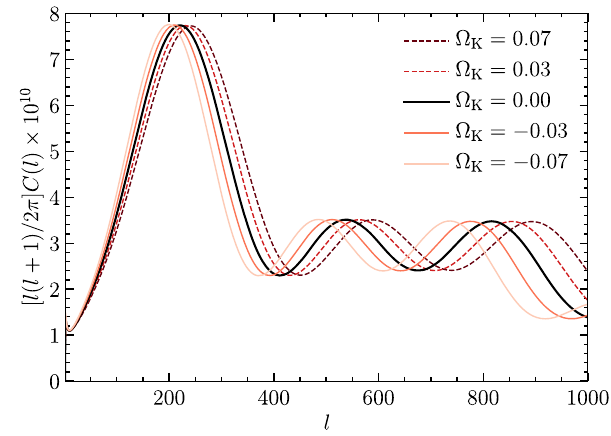
\includegraphics[width=0.8\textwidth]{img/curvatura.png}
    \caption{Effects of curvature parameter $\Omega_K$ on CMB temperature anisotropy power spectrum.}
\end{figure}

\begin{figure}[H]
    \centering
    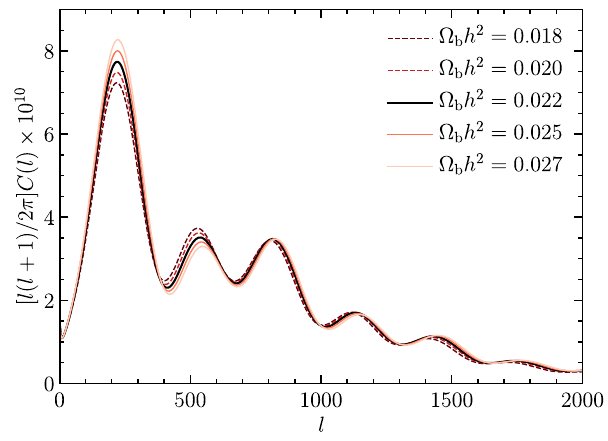
\includegraphics[width=0.8\textwidth]{img/baryon_density.png}
    \caption{Effects of baryon density parameter $\Omega_b h^2$ on CMB temperature anisotropy power spectrum.}
\end{figure}

\begin{figure}[H]
    \centering
    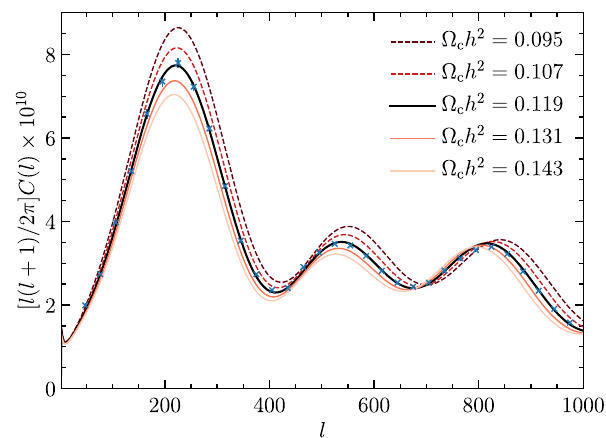
\includegraphics[width=0.8\textwidth]{img/cdm_density.png}
    \caption{Effects of CDM (cold dark matter) density parameter $\Omega_c h^2$ on CMB temperature anisotropy power spectrum; also shown are binned Planck 2018 measurements.}
\end{figure}

As promised just by inspecting the previous plots we appreciate that in general power spectra are indeed shaped by the values of cosmological parameters; this is the property exploited to replace complete likelihoods with just power spectra.


\subsection{Emulating the Planck 2018 Likelihood with \emph{CosmoPower}}
% cita il codice, il metodo get loglik dovrebbe bastare. Serve a dimostrare come funzioni in pratica CosmoPower nel contesto di come Planck approssimi la likelihood (riprendi discorso di prof e paper relativo agli approximation schemes):
% cosmopower fa la sua predizione per i C_ell corrispondenti all'input richiesto, poi tenendo conto del binning calcola la predizione finale; questa viene paragonata agli estimator dei C_ell ottenuti dai dati e li mette in una gaussiana con covarianza sempre stimata dai dati o comunque che lui legge da file. Ovviamente ha senso iniziare dicendo che Planck sceglie proprio Cl e pseudo Cl, che combina con una stima della covarianza (slide 143, ma mi pare ci sia scritto pure nella sezione sulle approssimazioni del paper)
To conclude this lengthy discussion we present an example that can effectively summarize everything discussed so far about using emulators in CMB experiments.

As discussed to explain equation \eqref{eq:approx_cmb} in realistic CMB analyses one must choose an approximation scheme for the original exact Gaussian likelihood; in particular one must choose $Z$ and $\hat{Z}$ (functions of $C_\ell$ and $\hat{C}_\ell$ used to replace them) and an appropriate covariance matrix. 
In the case of the \emph{Planck 2018} data analysis \cite{planck_2018} the complete inference pipeline was as follows:
\begin{itemize}
    \item The $C_\ell$ and the pseudo-$C_\ell$ themselves were chosen, i.e. $Z$ and $\hat{Z}$ are the identity function;
    \item The pseudo-$C_\ell$ were extracted from the data in the cut-sky regime;
    \item Accurate simulations of the actual dataset were built assuming a fiducial cosmological model;
    \item The pseudo-$C_\ell$ were measured using these simulations; from their MCMC averages the covariance matrix was estimated;
    \item Finally compute the difference between observed and predicted $C_\ell$'s, then use this difference and the above covariance matrix to build the usual exponential-of-quadratic-form Gaussian functional form.
\end{itemize}
Essentially this approach is almost the same as the exact one (i.e. a Gaussian likelihood containing the difference between predicted and experimentally estimated power spectra), with the only difference that the covariance matrix was obtained with complex simulations based on theoretical techniques.

Assuming that a) the $\{\hat{C}_\ell\}$ dataset has been extracted from raw experimental data, and that b) the covariance matrix has been computed, then the only non fixed part of the likelihood is the theoretical prediction of the $C_\ell$'s.
This is consistent with the Bayesian approach to statistics: the data is collected at the beginning and set in stone, while the parameters are allowed to vary to e.g. sample different values of the posterior. 

Accelerating these evaluations of the $C_\ell$'s (that would otherwise require expensive exact solvers) was precisely the reason why \textsc{CosmoPower}; it is particularly informative to show a code snippet from \textsc{CosmoPower}'s source to show how the emulator interfaces with the steps above.
\lstinputlisting[language=Python, caption={The code \textsc{CosmoPower} uses to compute the \emph{Planck 2018} likelihood using its internal emulators; code snippet taken from \textsc{CosmoPower}'s source.}]{code/cosmopower_planck2018_likelihood.py}
The above code has been taken as-is from \textsc{CosmoPower}'s source, without even modifying the comments; the only edit performed was to discard irrelevant parts.

From this code snippet we can easily understand how \textsc{CosmoPower} computes the requested value of the Planck 2018 likelihood using emulators to speed up the process. In particular \textsc{CosmoPower} is used to obtain the emulator's predictions of the $C_\ell$'s corresponding to the requested parameters, \emph{for the same $\ell$ values contained in the Planck data} (lines 13-15); then, after some preprocessing needed to comply with the Planck dataset (lines 18-28) the log-likelihood is simply computed as the quadratic form of the difference between predicted and observed $C_\ell$ (lines 34-39) using the pre-computed covariance matrix (line 4).
This procedure is perfectly in line with the Planck 2018 likelihood's requirements; at the same time it clearly shows how the theoretical predictions of the $C_\ell$'s (for fixed $\ell$, variable cosmological parameters) can be replaced with the much faster emulator-based evaluations.


\section{Supernovae}
% valuta un po'. Penso basti essere più schematici: lo scopo di capire cosa siano i power spectra, perché siano utili (equivalenza con la likelihood, dipendenza dai parametri cosmologici) e perché si prestino all'emulazione (dipendenza regolare/liscia dai parametri) è stato raggiunto con la sezione precedente. Per questo penso basti definire ciò che viene usato nel notebook (luminosity distance, eccetera, capitolo 2 del libro come diceva il prof), e ripetere che le proprietà simpatiche appena scritte (dipendenza liscia e significativa dai parametri cosmologici) valgono anche in questo caso, tanto che sono state usate nel 1998 per scoprire l'accelerazione dell'espansione dell'universo... magari citi quel paper, come suggeriva il prof

\emph{Type Ia Supernovae} are astrophysical objects of great importance in observational cosmology; the reason for this is twofold. On one hand they are so bright that they can be seen from distances of cosmological scales; on the other they are \emph{standard candles}, i.e. their absolute magnitude (i.e. luminosity at the source) is \emph{constant}.\footnote{This is not exactly true: there are some fluctuations that must be accounted for before we can actually assume fixed source luminosity. See for example \cite{supernovae_bhm}, a study which also pioneered the use of Bayesian hierarchical modelling in cosmology.} This means that by simply observing their \emph{apparent magnitude} (i.e. luminosity at the observer) we can relatively easily measure their distances. Considering that these distances are cosmological they are affected by effects regarding the universe as a whole; in particular it means that \emph{we can use them to build distributions from which it is possible to infer the values of cosmological parameters}.
Conceptually speaking this type of inference is analogous to the CMB case discussed before; therefore there is no need to go into the technical details - especially considering that in section \ref{sec:discovering_dark_energy} we will see an example of an inference of this kind.
It is exactly to aid the example in that section that it pays off to quickly summarize some results about the analysis of supernovae data; in particular we want to define quantities that will be used in that example.

This brief review is based on \cite{modern_cosmology}.

\paragraph{Scale Parameter $a$}
In the standard model of cosmology the universe expands over time; to quantify this effect the \emph{scale parameter} $a(t)$ is defined. $a(t)$ is a function growing over time and that quantifies how distances \emph{scale} as the universe expands. For example we can imagine defining a grid that expands uniformly as time evolves: points on the grid, which cor-
respond to observers at rest, maintain their coordinates (i.e. the \emph{comoving distance} between them remains constant);  the physical distance, though, is proportional to the scale factor, and therefore it \emph{does} evolve with Indeed in cosmology we have two general distances: the \emph{comoving} one (which is defined by the grid, and therefore by definition remains constant), and the \emph{physical} one (the one that is ideally measured with a rigid ruler, and that increases as $a(t)$ over time). 
Using General Relativity it is possible to compute how $a(t)$ evolves in time for a given spacetime geometry, assuming a certain composition of the cosmic inventory (e.g. a matter-dominated/radiation-dominated/dark energy-dominated universe); by definition this function quantifies the rate of expansion of the universe, and therefore depends on the precise values of cosmological parameters such as e.g. the curvature parameter $\Omega_K$.

\paragraph{Redshift $z$}
A consequence of the expansion of the universe it that \emph{the wavelength of light travelling over cosmological distances is increased}; this ``photon stretching'' effect is called \emph{cosmological redshift}. 
In particular since $\lambda\propto a$ we can quantify this stretching by introducing the \emph{reshift parameter $z$}:
\begin{equation*}
    1+z \equiv \frac{\lambda_{\text{observed}}}{\lambda_{\text{emitted}}} = \frac{a_{\text{observed}}}{a_{\text{emitted}}}
\end{equation*}
The redshift parameter is quite useful because it is easy to compute: by measuring the wavelength of received photons and comparing it with the (known) wavelength they were emitted with we can quickly obtain $z$, and with it the ratio between the scale factor today and at the time of emission. $z$ therefore represents an easy to measure quantity that can be used to gain information about the scale parameter $a$ in the past; in particular since $a$ grows over time \emph{$z$ can be used to measure the flow of time in an expanding universe}. Also since the light of farther away objects is subject to stronger redshift we remark that $z$ can be used to measure cosmological distances, too. The easiness with which $z$ can be computed, together with its several intuitive interpretations, make it an ideal tool in cosmology; indeed it is common to indicate the distance to a source by reporting the redshift of its emitted light.
In particular since by convention the scale factor today is set to 1 we can write that $a = 1/(1+z)$; this is then used to obtain the time of emission/distance to the source.

\paragraph{Angular Distance}
A classic way to determine distances in astronomy is to measure the angle $\theta$ subtended by an object of known physical size $l$ (``standard ruler''). Since this angle is usually small the distance to that object can be obtained as $d_A = l/\theta$, where by definition $d_A$ is the \emph{angular distance}, i.e. the distance measured through angles.
It is possible to show that depending on the considered geometry angular distance is related to the scale factor via the comoving distance; this is intuitive, since as we discussed before the scale factor measures how much the constant comoving distance should be scaled to match the always expanding physical one. 
The fact that the particular function relating $d_A$ and $a$ depends on the curvature parameter $\Omega_K$ can be used to infer its value.

\paragraph{Luminosity Distance}
Another way of inferring distances in astronomy is to measure the flux from an object of known luminosity (``standard candle''). For nearby objects, the flux $F$ observed at a distance $d$ from a source of known luminosity $L$ is $F=L/(4\pi d^2)$ since the total luminosity through a spherical shell with area $4\pi d^2$ is constant and equal to $L$.
This relation too can be generalized to cosmological scales and be related to the scale factor in a way that depends on the overall geometry of the universe; the details can be found in \cite{modern_cosmology}. The distance defined in this way (i.e. by comparing the observed luminosity with the one at the source) is called \emph{luminosity distance}.
For our purposes it suffices to state that by measuring this quantity we can infer cosmological parameters in another, independent way.


\paragraph{Distribution Of Distances}
Type Ia supernovae are standard candles, which means they are basically clones of the same template. Let us assume we observed a large number of them; by measuring the redshift and luminosity/angular distance of each one of them we are essentially sampling many times from the same likelihood, conditioned on the true values of the cosmological parameters. By inverting this relation we can use the obtained data to obtain a posterior describing the inferred parameters; showing a simplified version of this procedure is the purpose of section \ref{sec:discovering_dark_energy}.
This type of inference has always been fruitful; for example it was used in 1998 to discover the existence of \emph{dark energy}, which led to the 2011 Nobel prize in physics.
By using the concepts introduced in this brief section we will be able to gain considerable insight regarding this type of analyses.